    \section{Process' perspective}

% Taken from: https://github.com/itu-devops/lecture_notes/blob/39aaac80478c8f90870269760864ff32c23b5cce/REPORT.md
% OBS: THIS IS THE REPORT TEMPLATE FROM LAST YEAR

% Process' perspective

% A description and illustration of:

%     How do you interact as developers?
%     How is the team organized?
%     A complete description of stages and tools included in the CI/CD chains.
%         That is, including deployment and release of your systems.
%     Organization of your repositor(ies).
%         That is, either the structure of of mono-repository or organization of artifacts across repositories.
%         In essence, it has to be be clear what is stored where and why.
%     Applied branching strategy.
%     Applied development process and tools supporting it
%         For example, how did you use issues, Kanban boards, etc. to organize open tasks
%     How do you monitor your systems and what precisely do you monitor?
%     What do you log in your systems and how do you aggregate logs?
%     Brief results of the security assessment.
%     Applied strategy for scaling and load balancing.

% In essence it has to be clear how code or other artifacts come from idea into the running system and everything that happens on the way.

\subsection{Interaction as developers}
Communication and interaction between team members have been moderately split between informal, formal, synchronous and asynchronous communication throughout the entire course. Initially Microsoft Teams and Github issues were used. As we later experience Microsoft Teams to not be sufficient and fitting for the team, we moved to using Discord instead of Microsoft Teams.




%Communication and interaction between team members have been moderately split between informal, formal, synchronous and asynchronous communication throughout the entire course. Initially we used Microsoft Teams and GitHub issues for asynchronous, formal and informal communication. However, we quickly realised that teams would not be an applicable solution for our project. This realisation came as a consequence of team members not responding/not being active on teams for several days (even when we faced an imminent problem that caused our application to unexpectedly go offline!). Consequently, we looked into alternative solutions and decided that Discord would be a much better option, since the majority of the team were quite frequently online on Discord and thus would be easier to reach.\\

%In regard to synchronous interaction and communication, we decided that team meetings would be held on Tuesdays after the lecture. The meetings would usually cover three topics: the distributed work we did the previous week, what needs to be accomplished to reach this week's milestone and finally how the issues for this week would be distributed between team members. In continuation of these meetings, we would work closely together for several hours and these sessions would be based on pair/mob programming, where we would try to solve the current week and last week's issues together. Furthermore, we also had several distributed meetings on teams and discord. These meetings would follow the same work ethic as the physical ones.\\

%Regarding the social atmosphere in the group, it can easily be said that we have high psychological safety, in the sense that team members are not afraid to speak up and voice their opinions. In general, this made the process much more fun and interactive and also contributed to a more solid teamwork and project. The main ethic behind delivering code and generally working on the project is full transparency, i.e it should be easy to continue to work on tasks that are not yet finished. This was mainly accomplished by documenting the work done on the issue at hand, but also through the weekly team meetings.

\subsection{Team organisation}
The team is organised with all members having equal authority. Project scope and project requirements are set by Helge and Mircea, as well as extra needs requested by the group. 

\subsection{Description of CI/CD chains}
%A complete description of stages and tools included in the CI/CD chains
%- That is, including deployment and release of your systems.
Github Actions is used for CI. TravisCI was initially used, since this was well-documented and also separated the deployment from the codebase by not having everything at Github (see issue see issue \href{https://github.com/DevelOpsITU/MiniTwit/issues/58}{\#58}). However, as the free plan on TravisCI expired, CI chain was moved to Github actions, as developers were familiar with this, as well as Github actions providing a faster pipeline (mainly spinning up VM's) (see issue see issue \href{https://github.com/DevelOpsITU/MiniTwit/issues/117}{\#117}).\\

\subsubsection{CI Chain}
CI chain is setup according to the operation on branches (see issues see issue \href{https://github.com/DevelOpsITU/MiniTwit/issues/69}{\#69} and see issue \href{https://github.com/DevelOpsITU/MiniTwit/issues/117}{\#117}), such as seen in \autoref{fig:CIChain}: 
\begin{figure}[H]
    \centering
    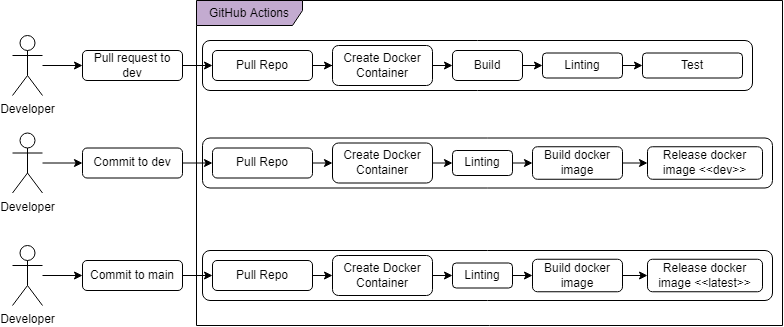
\includegraphics[width=\linewidth]{images/diagrams/CI_Chain.png}
    \caption{Different GitHub actions}
    \label{fig:CIChain}
\end{figure}
%\begin{itemize}
%    \item Pull request to dev
%    \begin{itemize}
%        \item Linting, build tests and system test
%    \end{itemize}
%    
%    \item Commit to dev (merge request accepted)
%    \begin{itemize}
%        \item Linting, build docker image, test docker image, publish with dev tag
%    \end{itemize}
%    
%    \item Commit to main (merge request accepted)
%    \begin{itemize}
%        \item Linting, build docker image, test docker image, publish with latest tag
%    \end{itemize}
%\end{itemize}

An example of the "pull request to dev" CI run can be seen at GitHub \cite{ci_run_example_1}.
The Linting tools used are Go lint\cite{golinter.sh}, for linting the application code, Shellcheck \cite{shellchecker.sh}, for linting all scripts. After Linting and testing, scancode \cite{scancode_dockerfile}, scans for licenses, however, the result is not actually used, since it has been commented out in the yml file\cite{pullreq_to_dev_yml}. For the other chains if everything passes, a docker image is build, linted using hadolint\cite{hadolint} and released. \\

Besides these GitHub actions SonarCloud is setup to run static analysis of the changes, and describe if code has become worse with the pull-request. Git Guardian, also checks for vulnerabilities, leaked passwords etc.


%Code linting, code analysis, vulnerability checks (see issue see issue \href{https://github.com/DevelOpsITU/MiniTwit/issues/113}{\#113})
%SonarCloud (see issue see issue \href{https://github.com/DevelOpsITU/MiniTwit/issues/114}{\#114}). 


\subsection{Organisation of repositories}
%- That is, either the structure of of mono-repository or organization of artifacts across repositories.
%- In essence, it has to be be clear what is stored where and why.

The project is split up into three repositories.\cite{contributing.md}
\begin{itemize}
    \item minitwit (main application)
    \item minitwitdevelopment (docker containers for use in development environment)
    \item serverdeployment (files for setup and maintenance of server applications)
\end{itemize}


\subsection{Applied branching strategy}
\begin{table}[h]
\begin{tabular}{|
>{\columncolor[HTML]{ffffff}}l |
>{\columncolor[HTML]{ffffff}}l |}
\hline
main & \begin{tabular}[c]{@{}l@{}}used as base branch, from which releases are created. \\ this must always be buildable and runnable.\end{tabular}                                                                                                    \\ \hline
dev  & \begin{tabular}[c]{@{}l@{}}used for development. \\ this must always be buildable and runnable. \\ every branch (except main) is derived from this branch.\end{tabular}                                                                         \\ \hline
*    & \begin{tabular}[c]{@{}l@{}}branches derived from dev have the following templates, depending on the issue's topic:\\ - features/\#(issueid)-(issue\_title / relevant\_title)\\ - bugs/\#(issueid)-(issue\_title / relevant\_title)\end{tabular} \\ \hline
\end{tabular}
\caption{branching strategy \cite{contributing.md}}
\label{tab:branching_strategy}
\end{table}

An example of the branching strategy applied, can be seen on \autoref{fig:github_network_graph}, where the green, purple and yellow all are feature branches. They are all branched out from the dev branch, and any merge conflicts should be handled in the feature branch, before doing a pull request back to dev.

\begin{figure}[H]
    \centering
    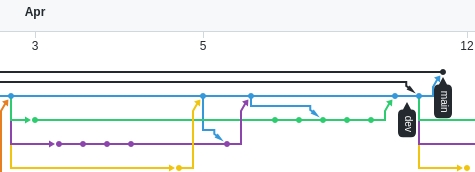
\includegraphics[scale=0.5]{images/diagrams/github_screenshots/github_network_graph_white.jpg}
    \caption{Github network flow graph}
    \label{fig:github_network_graph}
\end{figure}



\subsection{Applied development process}
%Applied development process and tools supporting it
%- For example, how did you use issues, Kanban boards, etc. to organize open tasks

For issues, Github's own issue management is used. Most issues are created and managed in \textit{MiniTwit} repository for simplified structure and readability. Issues are then assigned to individual members, whom are responsible for the issue (with assistance from other team members). \\
Commits are expected to happen regularly and to be descriptive. The commits' subject is limited to 50 chars, with few exceptions. Large commits are to be described in bulletpoints. \\
Pull-requests are to not be reviewed by the author himself, but by one more team members. \cite{contributing.md} \\






\subsection{Monitoring of MiniTwit}
%How do you monitor your systems and what precisely do you monitor?

To monitor MiniTwit is the visualisation tool Grafana used. Grafana can pull data from various sources and display it on dashboards, which can have different focuses. The reasons to choose Grafana can be found in issue \href{https://github.com/DevelOpsITU/MiniTwit/issues/100}{\#100} and are summarized here below:

\begin{itemize}
    \item Free
    \item Previous experience
    \item Extensive documentation
    \item Integrates well with many different data sources
    \item Works well with Loki\footnote{will be described later}
\end{itemize} 


To gather data from different services have Prometheus been deployed, its a tool that pulls data from services that offers a /metrics endpoint. The reason for why Prometheus have been chosen can be found in \href{https://github.com/DevelOpsITU/MiniTwit/issues/99}{\#99} and is summarised here below:

\begin{itemize}
    \item Free
    \item Previous experience
    \item Extensive documentation 
    \item Many library \gls{api} interactions
    \item Integrates well with Grafana
\end{itemize} 

The process and flow of data can be seen in \autoref{fig:Grafana_Data_Sourcing}. The users query Grafana which then queries both, or Prometheus and PostgreSQL. Prometheus continuously pulls data from the different servers and applications, which provides a metric endpoint. 

\begin{figure}[!ht]
    \centering
    \captionsetup{justification=centering,margin=1cm}
    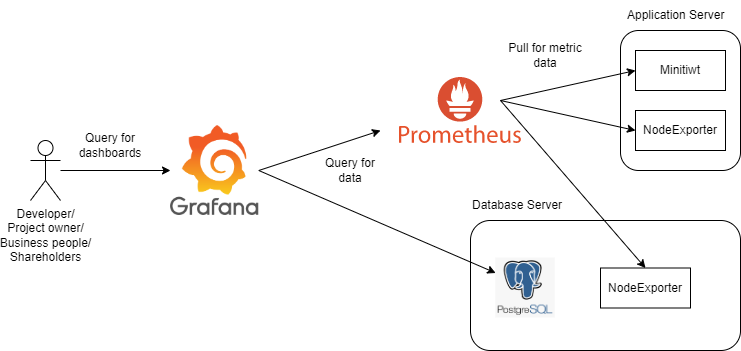
\includegraphics[width=120mm]{images/monitoring/MetricDataPulling.png}
    \caption{Grafana and Prometheus data sourcing process. (Source: own image)}
    \label{fig:Grafana_Data_Sourcing}
\end{figure}


Monitoring is used to provide information about: Business Intelligence, Endpoints, Server instances and the Simulator. (See Appendix \ref{app:grafana_dashboards} for visual of graphs and described in issues: \href{https://github.com/DevelOpsITU/MiniTwit/issues/103}{\#103},  \href{https://github.com/DevelOpsITU/MiniTwit/issues/121}{\#121},
\href{https://github.com/DevelOpsITU/MiniTwit/issues/124}{\#124},
\href{https://github.com/DevelOpsITU/MiniTwit/issues/126}{\#126} and 
\href{https://github.com/DevelOpsITU/MiniTwit/issues/151}{\#151})\\
\todo{heatmaps (issue 135)}

All monitoring information can be viewed at three endpoints: \textit{grafana.thomsen-it.dk}, \textit{prometheus.thomsen-it.dk} and \textit{monitoring.thomsen-it.dk} (See issue \href{https://github.com/DevelOpsITU/MiniTwit/issues/105}{\#105}).
\todo{Maybe find newer photos of updated dashboards}

As a combination with the monitoring system, alerts are set up via discord to notify of severe changes in data. Currently only Disk space, Ram usage, Response time and significant increase in Errors are setup with alerts (see issue see issue \href{https://github.com/DevelOpsITU/MiniTwit/issues/150}{\#150}).


\subsection{Logging of MiniTwit}
%What do you log in your systems and how do you aggregate logs?
Logging of the application follows the structure: \\
$\{"level":"info","time":"2022-03-04T16:48:07Z",\\"message":"Starting\: MiniTwit\: application\: startup\: checks"\}$ (See appendix \ref{app:logging_structure} and issue \href{https://github.com/DevelOpsITU/MiniTwit/issues/90}{\#90}).\\

For logging we use Loki, which is a log aggregation system, that is inspired by Prometheus\cite{grafana_loki}\cite{grafana_loki_docs}. Since it is inspired by Prometheus and also started at Grafana Labs, it integrated well with Grafana, aswell as developers already having experience with Prometheus from previous and current project. 

\subsection{Security assessment}
% Christian
%Brief results of the security assessment.
In lecture 9, the group were tasked with doing a security assessment with pentesting tools, which resulted in the work described in \autoref{app:security_ass} and in the Minitwit Github repo's wiki.\cite{}  


\subsection{Applied strategy for scaling and load balancing}
The application server is scaled by having two application servers hosted. To manage these two, a load balancer is setup up to direct traffic between them (see issue \href{https://github.com/DevelOpsITU/MiniTwit/issues/175}{\#175}. \\
The use of load balancer and two application servers also supplies the purpose of blue green deployment, such that one server at a time can be taken down, updated and put back online. This guarantees that at least one server will be active at all times.  \cite{blue_green_deployment}.

